% !TeX spellcheck = en_US
% !TEX root = ../thesis-example.tex
%
\chapter{Introduction}
\label{sec:intro}

\cleanchapterquote{If a technological feat is possible, man will do it. Almost 
as if it's wired into the core of our being.}{Motoko Kusanagi}{(Ghost in the 
Shell)}

Extending reality with the help of computer-generated imagery is no new 
concept. Ever since real-time 3D graphics was possible there was an attempt to 
extend the understanding of reality. Within recent years there have been 
great successes in the industry, most notably in image augmentation was 
"Pokémon Go" with an estimated install base of 750 million downloads 
worldwide in June, 2017\cite{appannie:2017}. Just before this thesis 
started, Apple and Google showed off their consumer-ready hard- and software 
for augmented reality experiences.
\newline
Virtual Reality Head-Mounted Displays have had a similar push in sales with an 
approximate of 5.83 million sold devices, which range in sales price between 
80 - 900€ for a VR kit, covering from the very simple Google's Daydream View up 
to the very sophisticated HTC Vive\cite{erguerel:2017}. And these figures don't 
include the sales of Google Cardboards, which is approximated at around 80  
million units\cite{superdata:market-brief:2017}.
\newline
This generation of computer systems, which includes PC workstations, game 
consoles and smart phones, is finally sophisticated enough in computation speed 
and sensor-accuracy to allow low latency tracking, precise to just a few 
millimeters spanning over an recommended area of about 
$20m^2$\cite{htc:vive-manual:2016}.

\section{Overview}
\label{sec:intro:outline}

The idea of Virtual Reality (VR) and Head-Mounted Displays (HMDs) stems from a 
cultural need to slip into roles of foreign worlds. Through the advancing 
development of hard- and software over the last decades emerges a medium which 
has unmatched immersion and creates a unique, transforming experience into any 
imaginable environment.

VR and HMDs are now advanced enough for consumer markets --- but virtual 
reality stumbles at communicating the experience. Without having ever put on a 
VR-Headset it is nearly impossible to understand --- or even imagine --- what 
the virtual reality experience means and feels like. Any observer of VR, 
usually done by showing what the VR actor is seeing, will not be able to get an 
understanding of the importance and shift of reality perception without wearing 
the headset himself.
\newline
Showing the video output from an HMD as marketing material is contradicting 
with classic motion video productions. There is even only one famous example 
where the perspective of a First Person Shooter is reenacted, which was in the 
overwhelmingly negatively received Doom (2005) movie.

The VR industry, including but not limited to game developers, exhibition 
creators and creative studios is in need of better communication devices for 
their products that include more than the current headset wearer and allows 
for a similar immersive but adapted experience.
\newline
The next step in VR production is called "Mixed Reality" (MR) and uses an 
external camera with the same tracking hardware of the headset to produce a 
video signal that shows the real world actor with the surrounding virtual world 
around him. There are currently three main methods of producing MR footage --- 
only one of these allows for live compositing with highly accurate imaging 
results. This will be covered by this thesis.

\section{Problem Statement}
\label{sec:intro:problem}

Initially I will research motion video productions, computer generated imagery 
and color theory. This leads to the knowledge of implementing basic, 
interactive live motion video feeds.
\newline
The core aspect will be integrating a multitude of hardware in a software that 
allows for dynamic video compositing in 3D environments at runtime while a user 
is interacting with the Virtual Reality scene. This allows for an actor using 
the Vive HMD to be composited into the scenery from a third person view 
and it will look like he is surrounded by the virtual scenery. The essential 
difference compared to classic post production is, that this system is planned 
to operate on runtime, allowing additional observers to get an interesting 
composited imagery of the VR actor's experience.
\newline
An additional extension is to dynamically track the cameras position, allowing 
for dynamic camera movement and a freely moving actor. Further work goes into 
increasing the resulting composited image quality by removing artifacts from 
the video feed and recreating the lightning environment and transferring it to 
the actor's video feed. 

\section{Challenges \& Scope}
\label{sec:intro:challenges}

This thesis discusses the development and usage of a mixed reality setup inside 
a single PC and a single application.
\newline
It will highlight the core motion video production for mixed reality, as it 
differs from other MR setups by staying inside the programs boundaries, 
integrating natively with the engine. Initially a latency between video camera 
signal and the software has to be solved for, which changes the rendering 
pipeline significantly.
\newline
Another main pivot will be chroma keying in real-time rendering, as well as 
image reproduction from the chroma matting result. In detail there will be a 
discourse of layered image composition as result of fore- and background of the 
VR actor.
\newline
Lastly composition controls will be implemented, adding a color-correction 
layer to the input video, giving a more natural look to the actor inside a 
surrounding 3D environment.

Outside of the scope of this thesis will be green screen compositing, as it is 
used as basic tool --- the same goes for high-fidelity video matting, which 
would require its own research for accurate runtime results with little to none 
user guidance. 
\cite{gong:realtime-matting:2010}, \cite{gastal:shared-sampling:2010}

\section{Results}

The Mixed Reality pipeline is rather complex, but is structured in three 
components: Recreating virtual camera parameters from the real world camera, 
readjusting a time drift between real world camera and generated engine frames 
and image composition of all media (fig. \ref{fig:intro:results}).

\begin{figure}[htbp]
	\caption{System Setup}
	\label{fig:intro:results}
	\centering
	\begin{subfigure}[t]{\textwidth}
		\centering
		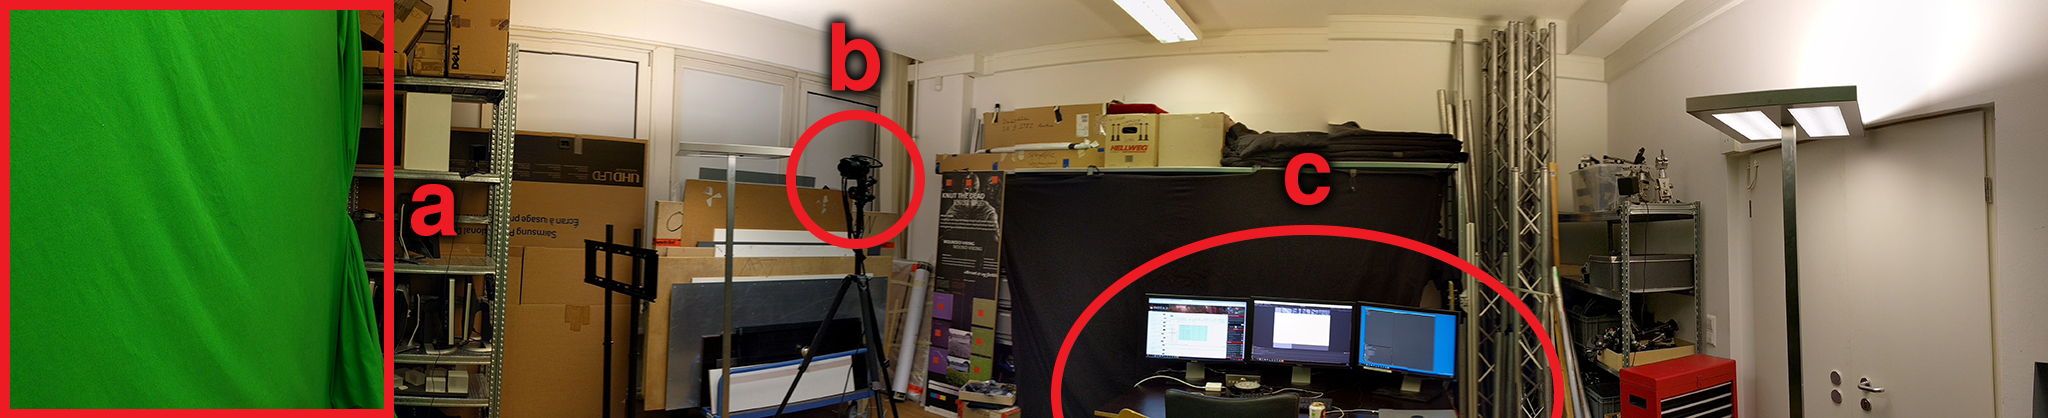
\includegraphics[width=\textwidth]{gfx/results/pano.png}
		\caption{Current studio setup --- \circled{a} green screen; 
		\circled{b} Panasonic Lumix GH2; \circled{c} PC Workstation}
	\end{subfigure}
	\begin{subfigure}[t]{.49\textwidth}
		\centering
		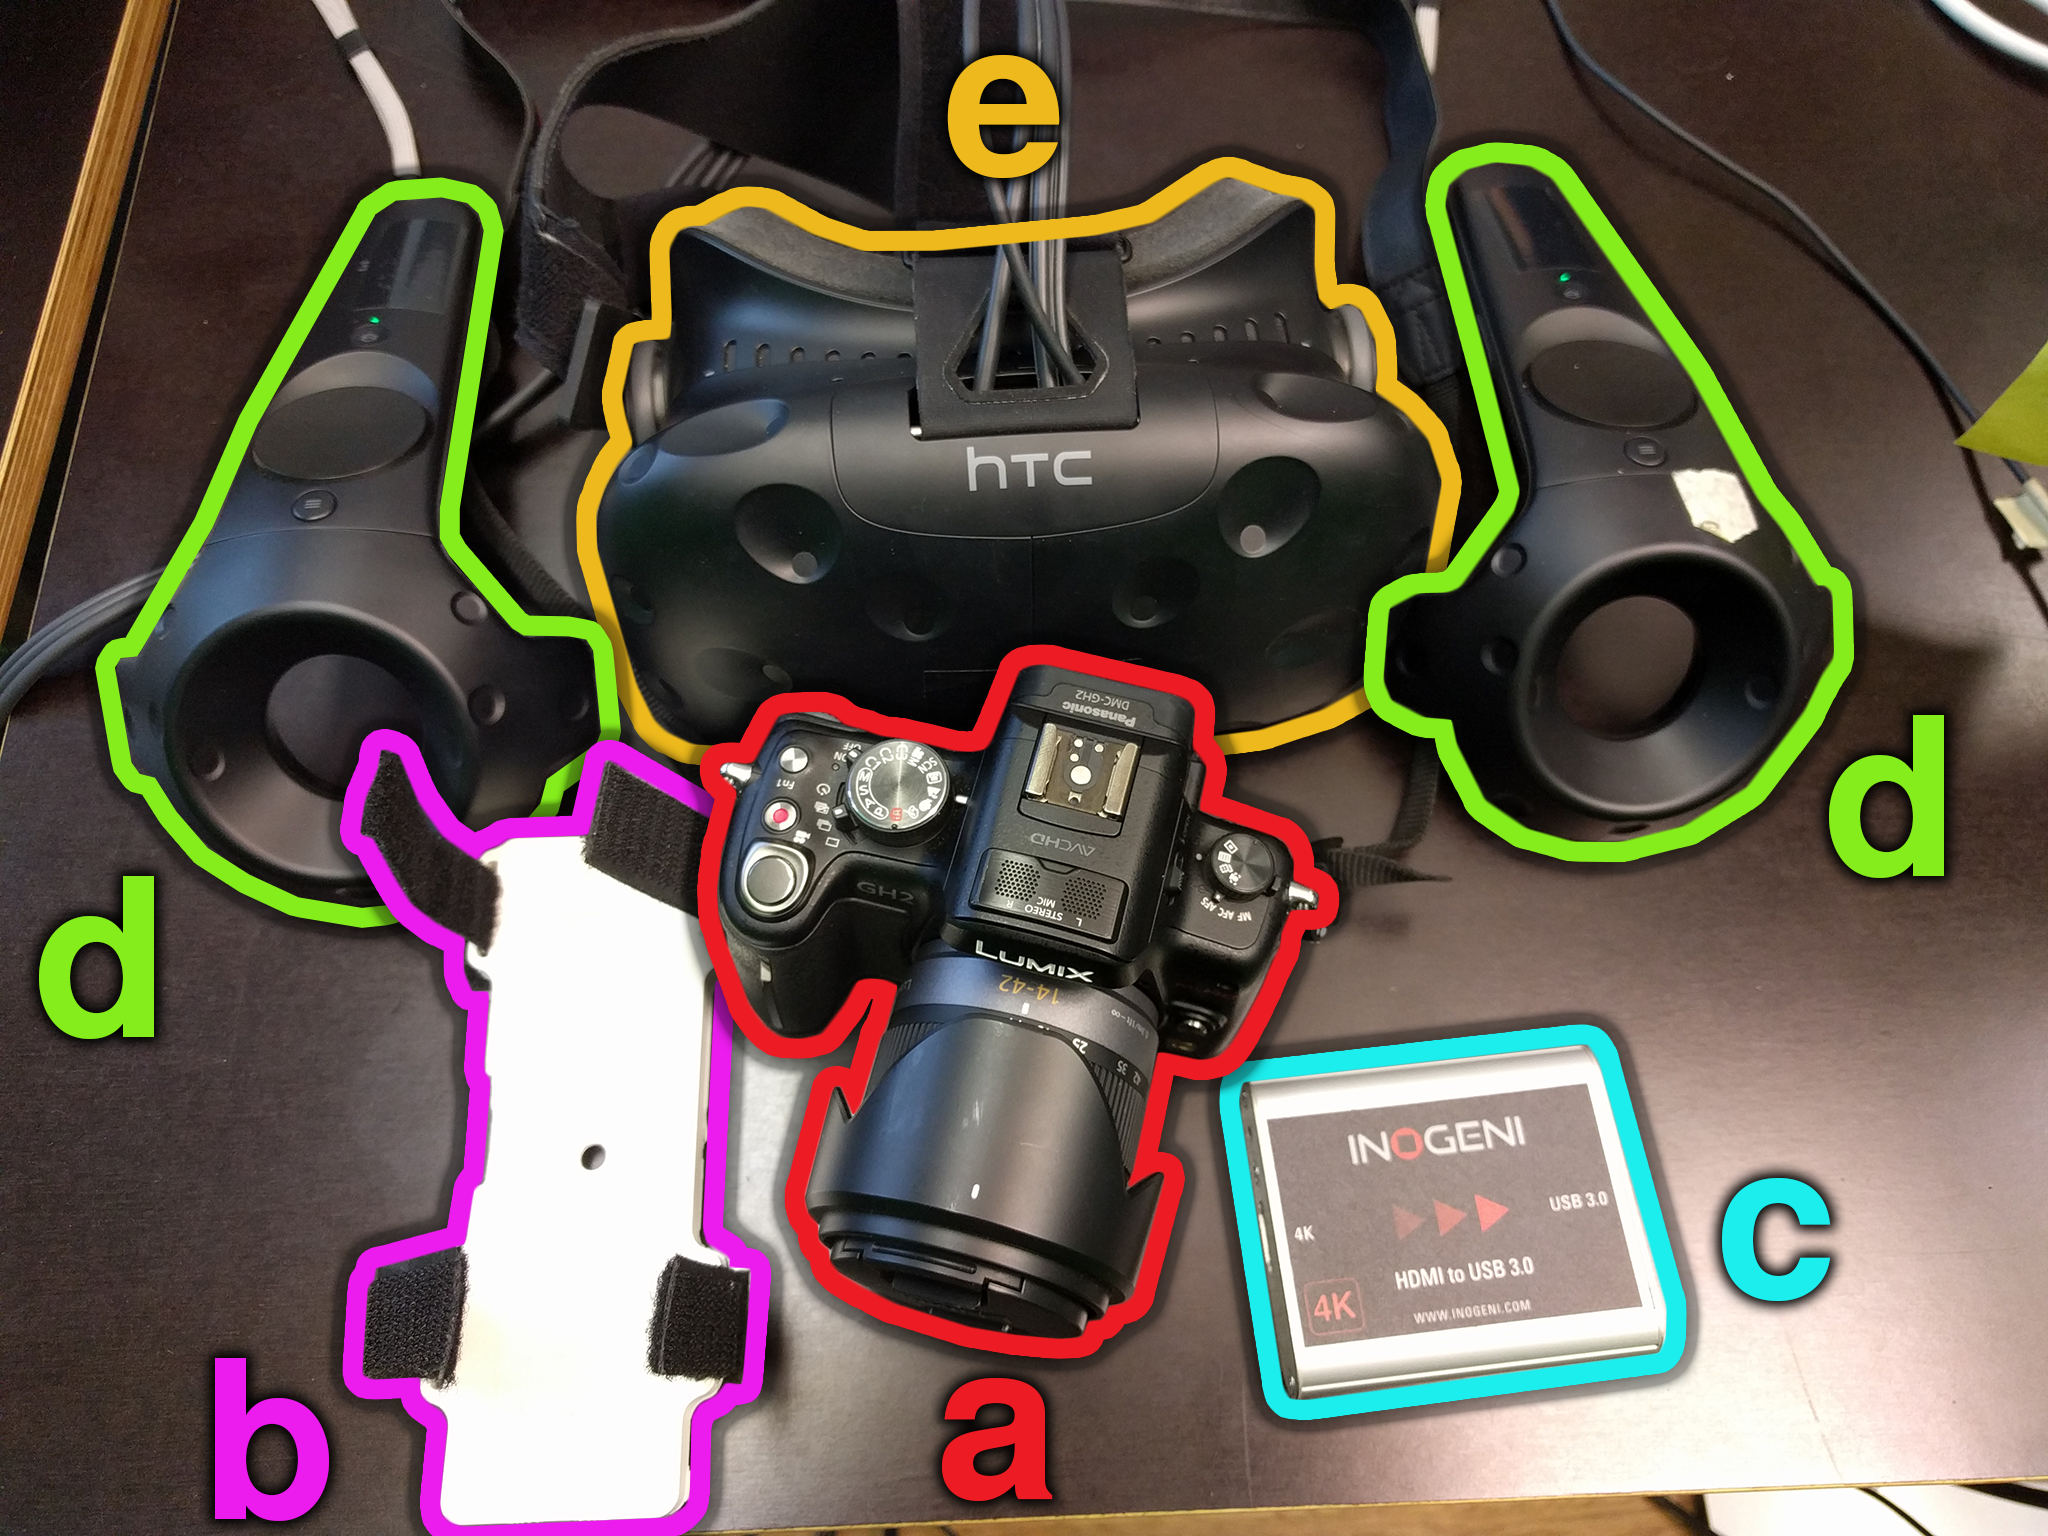
\includegraphics[width=\textwidth]{gfx/results/camera.png}
		\caption{System components --- \circled{a} Panasonic Lumix GH2; 
		\circled{b} Controller Tripod Mount; \circled{c} INOGENI 4KUSB3 HMDI 
		converter; \circled{d} HTC Vive Controller; \circled{e} HTC Vive HMD}
	\end{subfigure}
	\hfill
	\begin{subfigure}[t]{.49\textwidth}
		\centering
		\includegraphics[width=\textwidth]{gfx/results/set.png}
		\caption{\circled{a} Panasonic Lumix GH2; \circled{b} HTC Vive HMD; 
		\circled{c} green screen}
	\end{subfigure}
	\begin{subfigure}[t]{.49\textwidth}
		\centering
		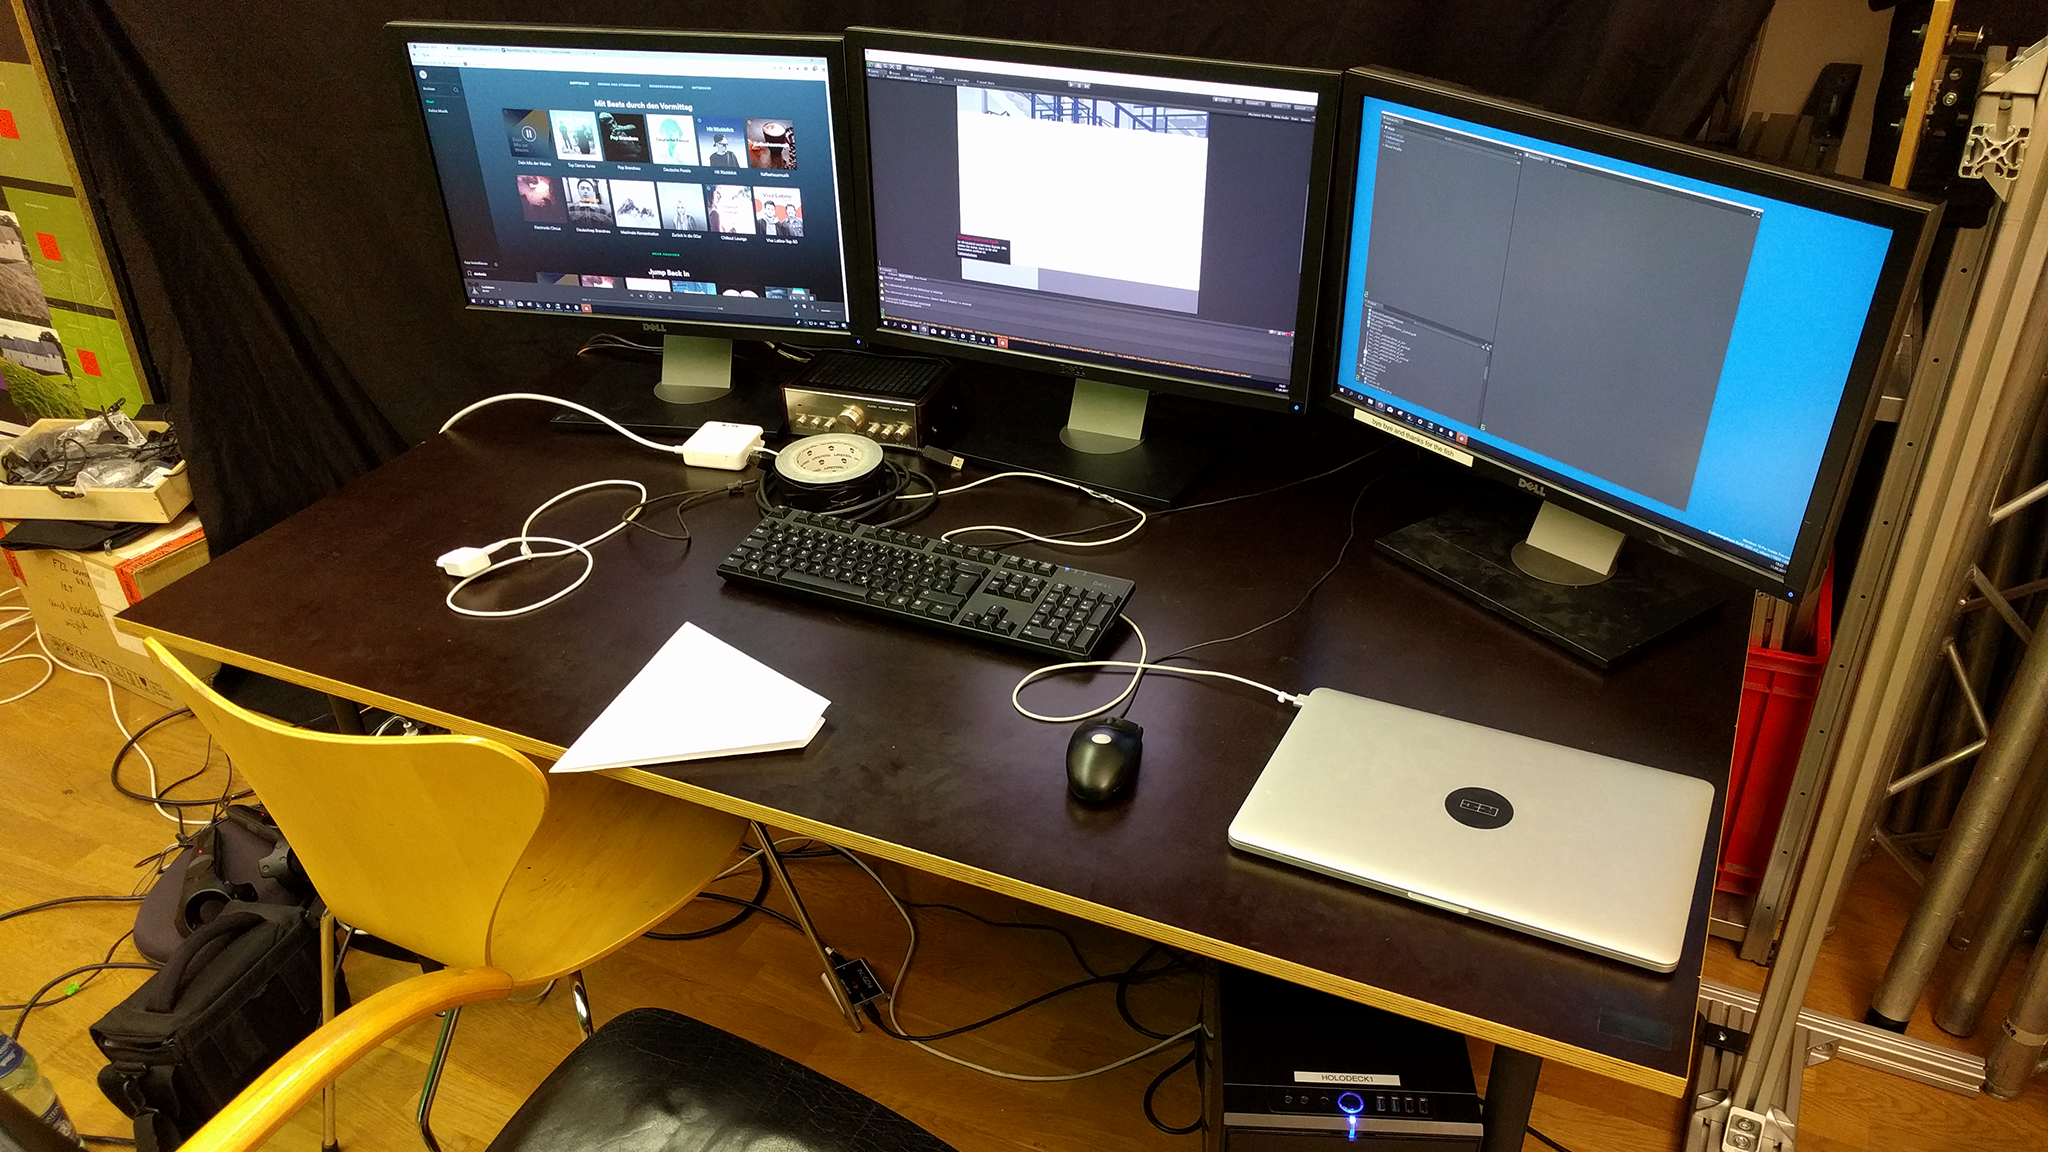
\includegraphics[width=\textwidth]{gfx/results/pc.png}
		\caption{PC Workstation}
	\end{subfigure}
	\hfill
	\begin{subfigure}[t]{.49\textwidth}
		\centering
		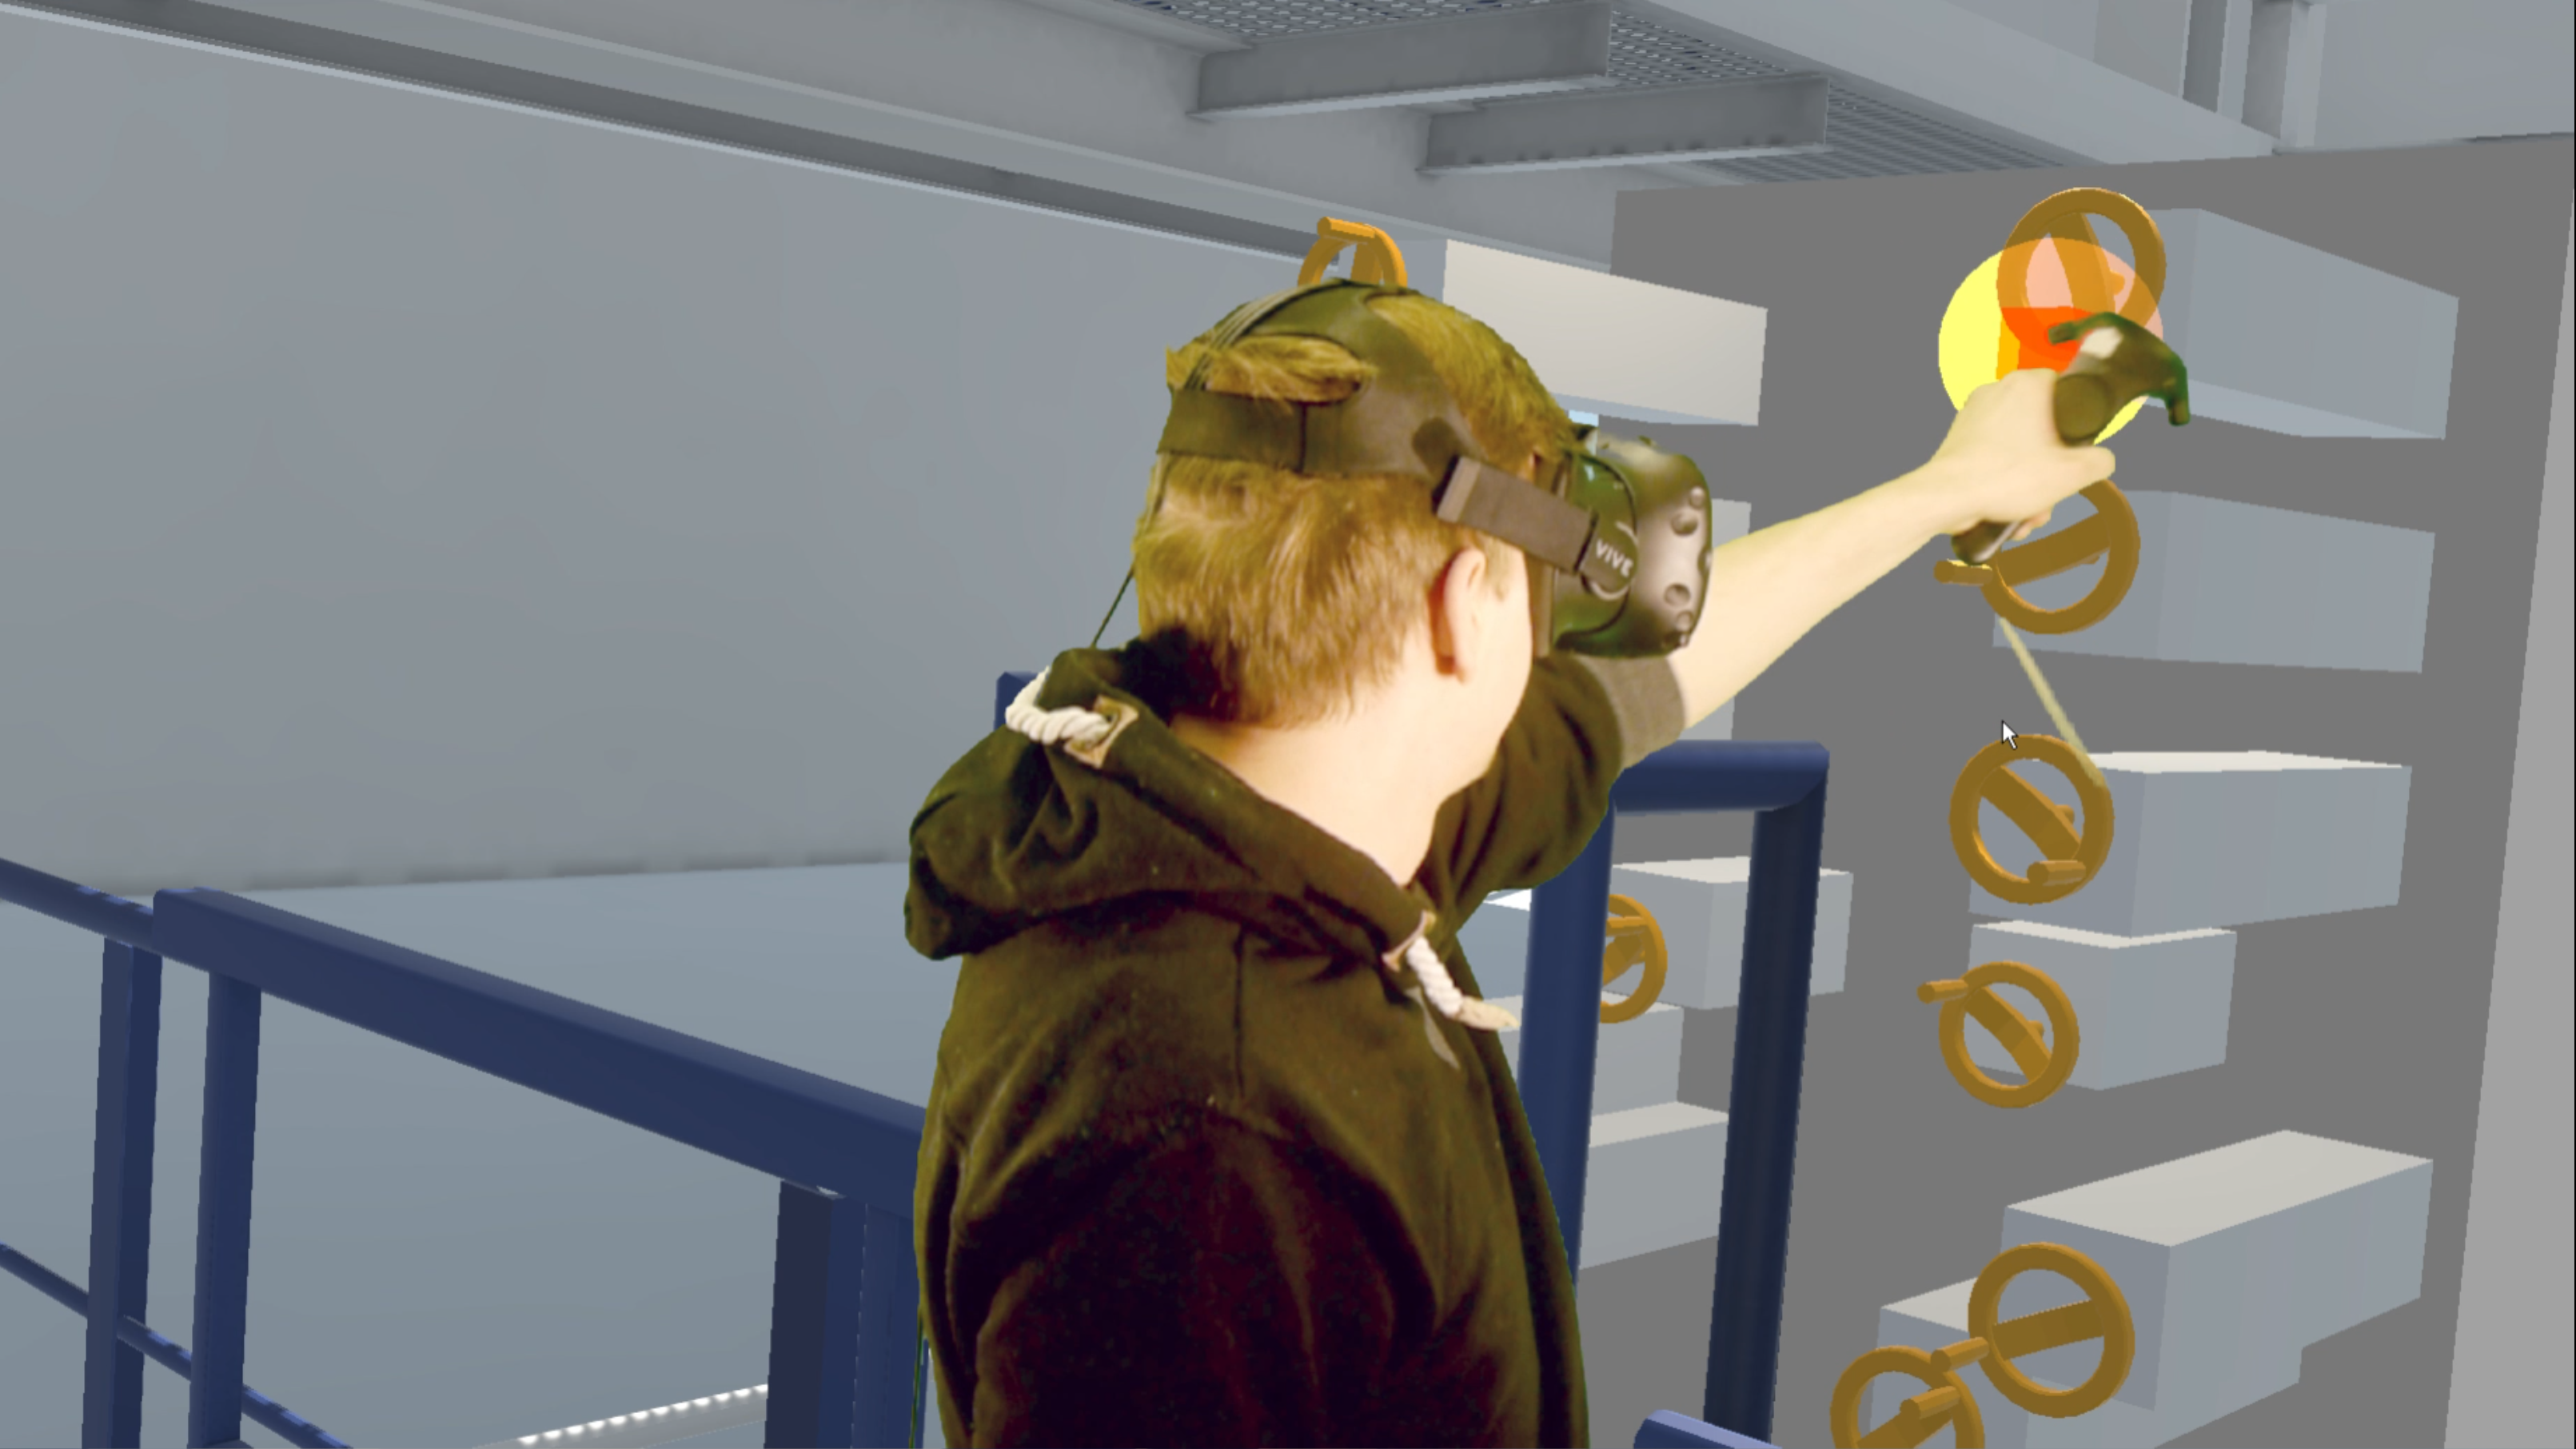
\includegraphics[width=\textwidth]{gfx/results/mr-action_new.png}
		\caption{final Mixed Reality composition}
	\end{subfigure}
	\begin{subfigure}[t]{.49\textwidth}
		\centering
		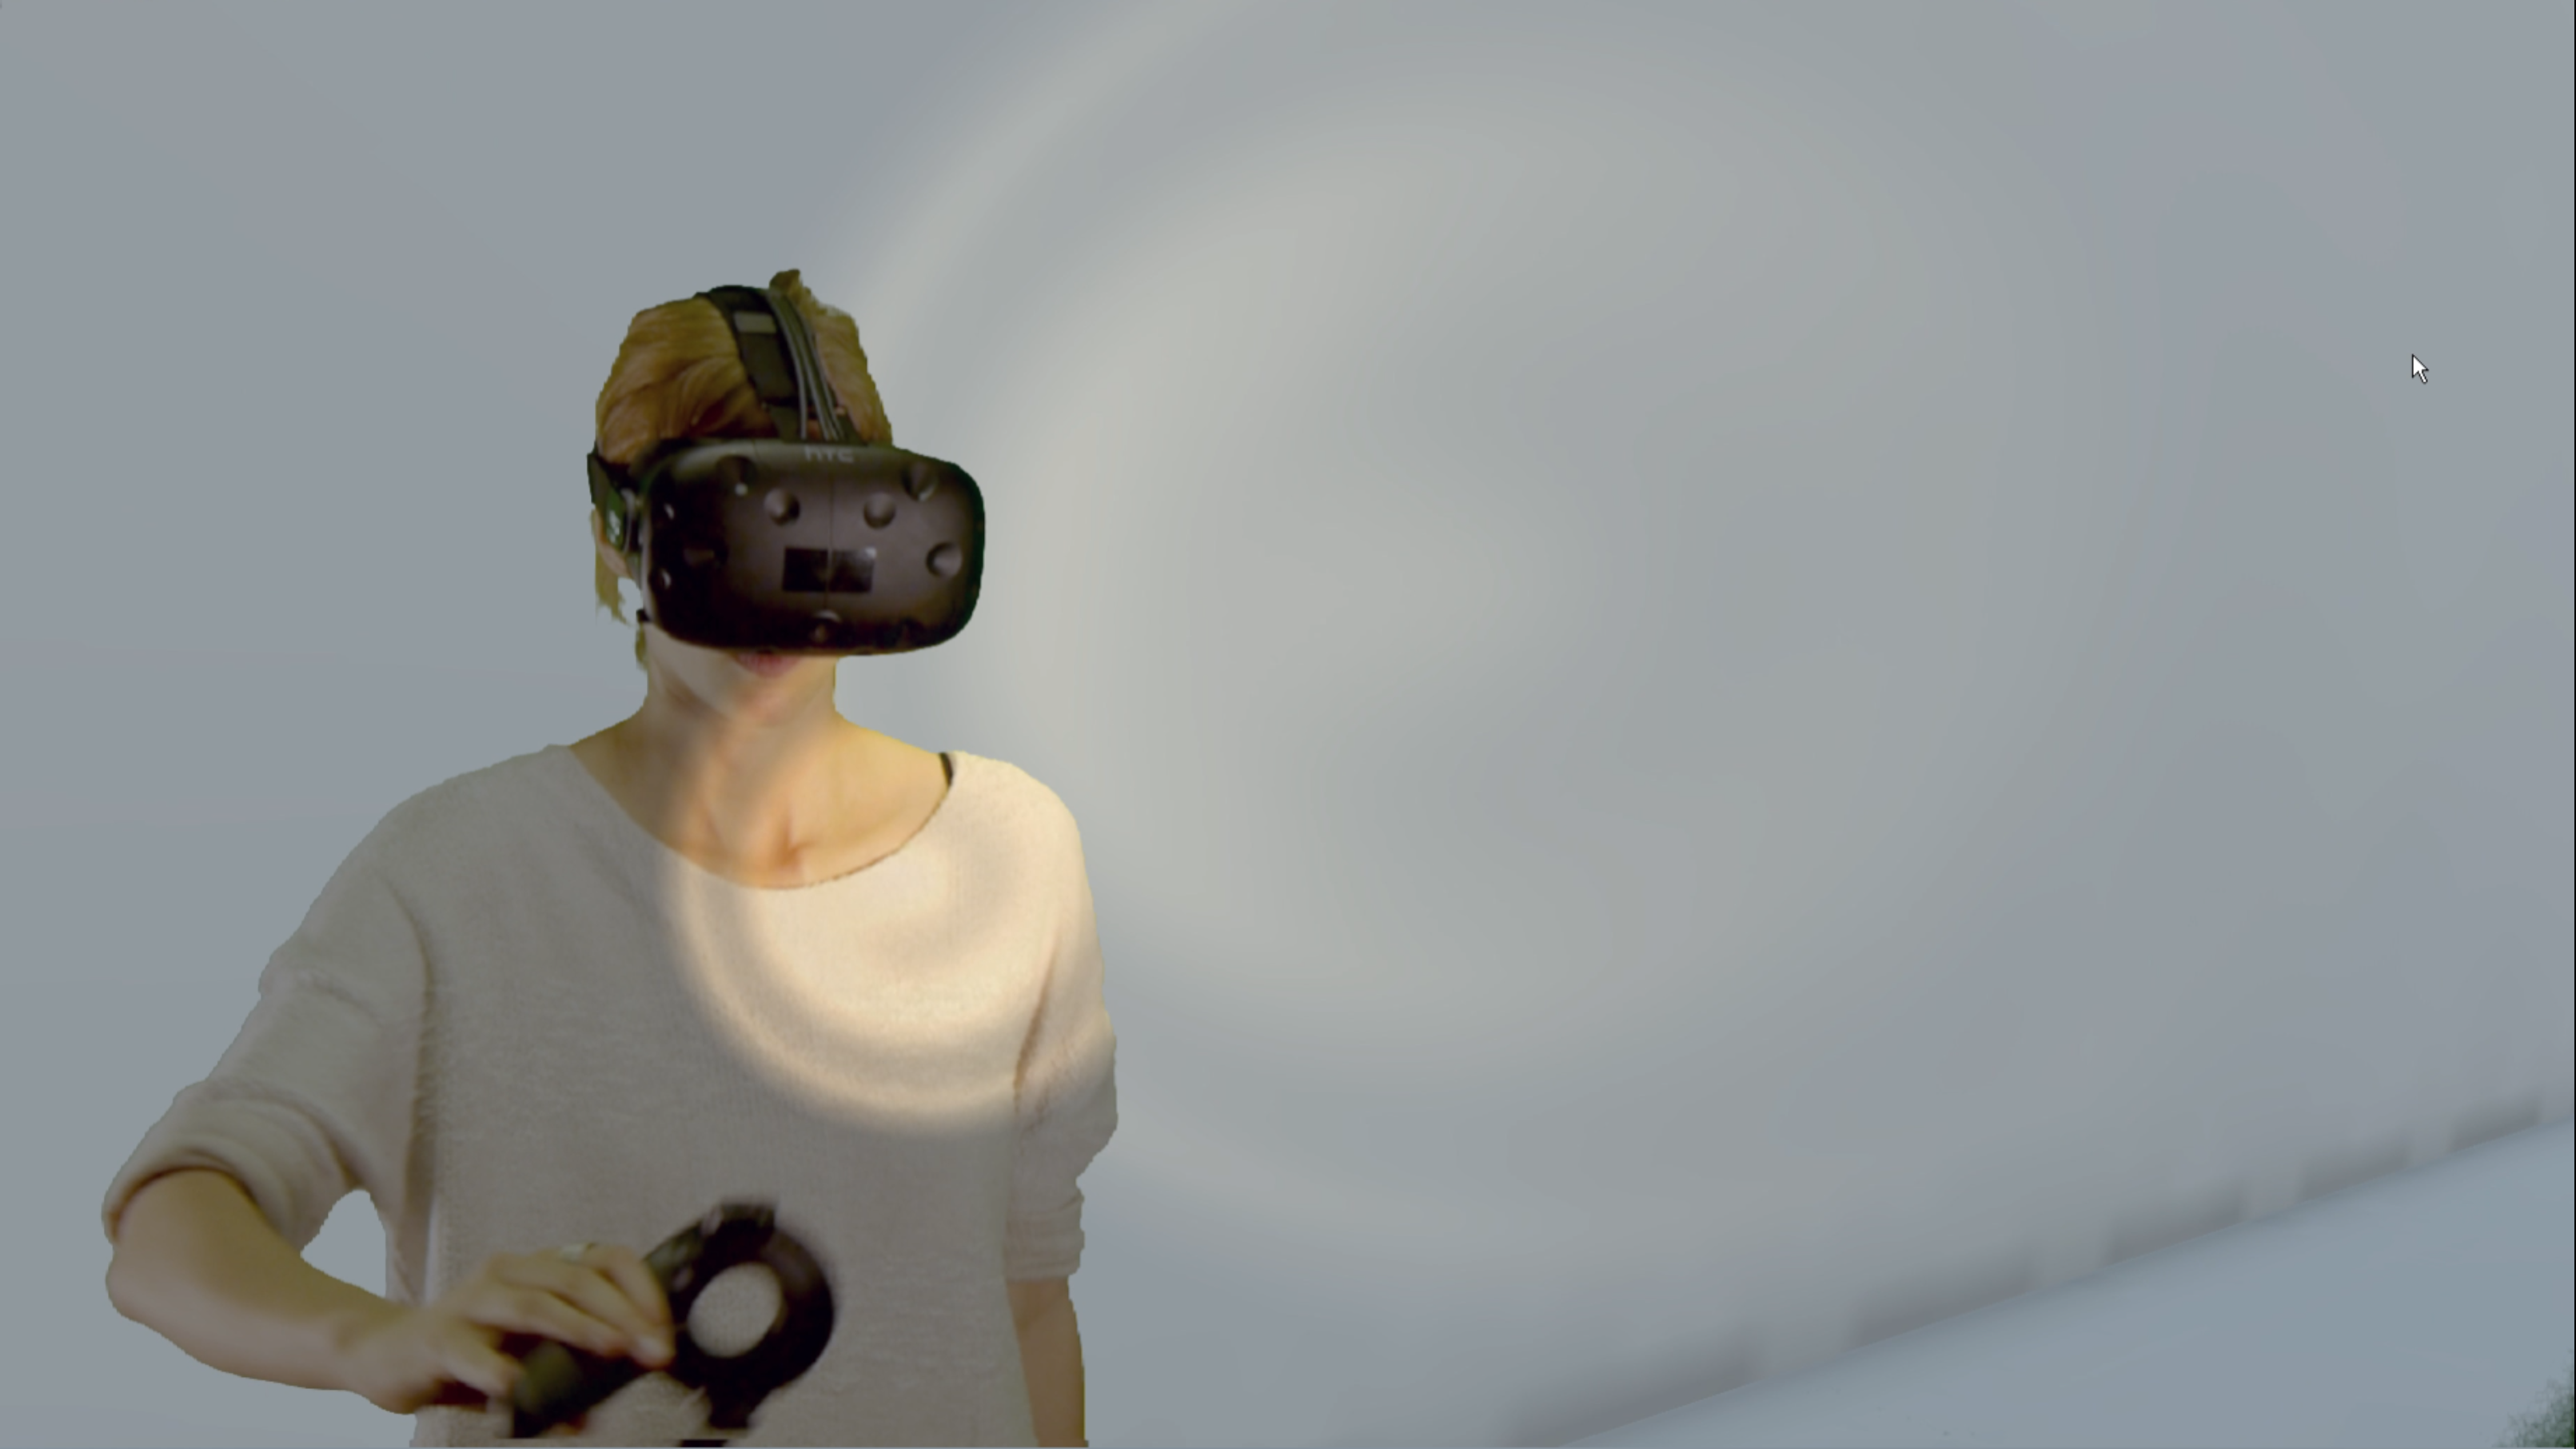
\includegraphics[width=\textwidth]{gfx/results/self-illu.png}
		\caption{Self-Illumination from virtual light casted on real world 
		camera image}
	\end{subfigure}
	\hfill
	\begin{subfigure}[t]{.49\textwidth}
		\centering
		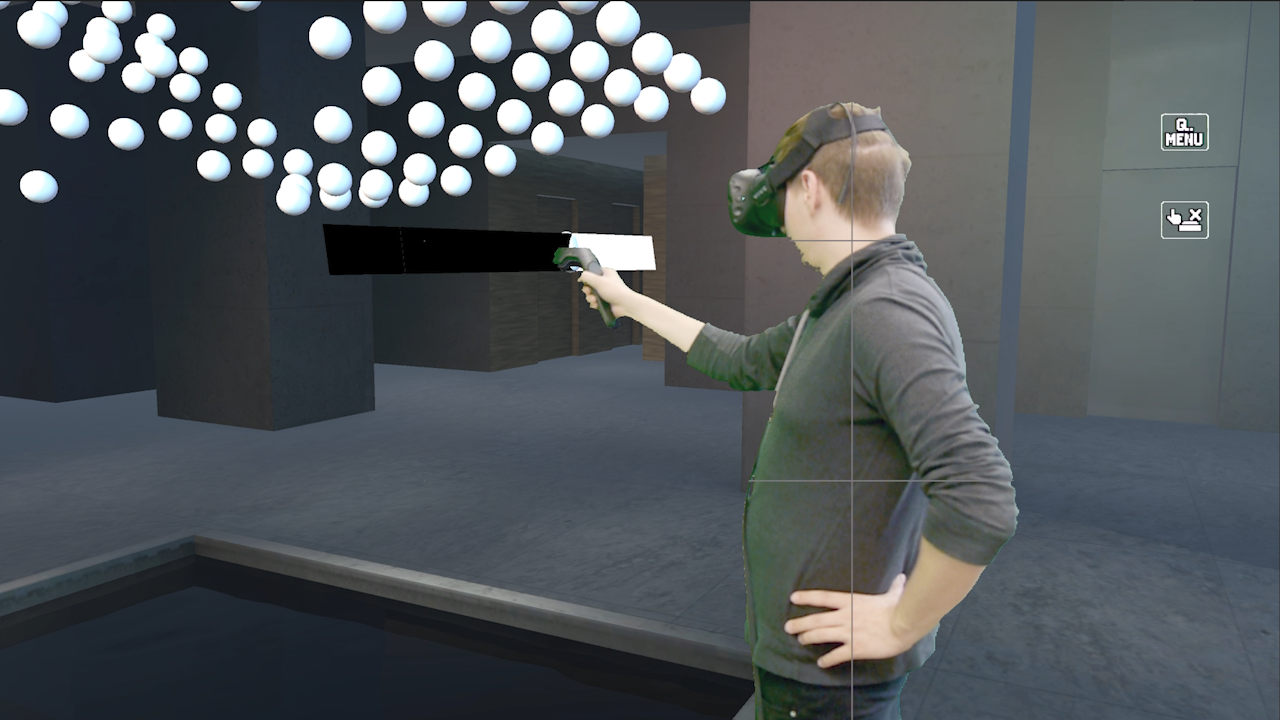
\includegraphics[width=\textwidth]{gfx/results/mr-action_old.png}
		\caption{another, earlier Mixed Reality composition}
	\end{subfigure}
\end{figure}

\section{Thesis Structure}
\label{sec:intro:structure}

At first an introduction to video production and different reality extending 
methods will be made. This discusses the history and current state of post- and 
live-productions to include a general overview of composition and production 
techniques.
\newline
This is followed by the application of this background knowledge to build a 
mixed reality pipeline, beginning from chroma keying, fixing input latencies, 
enabling virtual reprojection and more techniques.
\newline
Finally an evaluation and a conclusion will round up the discussed topics and 
highlight the discovered issues and future work.

This thesis gets completed by digital material hosted on GitHub. Print is a 
great medium, but lacks the ability for short demonstrations of video imaging 
solutions, problems and edge cases. To visualize these issues properly, all 
video media will have an annotation for cross referencing on the website. It is 
strongly suggested to follow these links for better understanding and 
highlighting of certain problems. They are sorted by chapters for easier 
navigation.

\section{Self Motivation}
\label{sec:intro:self-motivation}

My early teenage years started around the time when digitalization and global
interconnectivity begun and broadband Internet became commercially available.
Suddenly remote multiplayer games, unlimited image sharing --- and yes, music
sharing, too ---, Java-Applets, Flash, HTML framesets and "Marquee" CSS emerged 
in that medium. 3D Acceleration became a de-facto standard and even simple 
office PCs got weak, but dedicated graphics processing units built in, allowing 
for more complex user interfaces, animations and graphical fidelity. The mass 
of pixels by increasing the resolution of displays was basically a yearly 
iteration in greater, better, smaller, denser and brighter.

I am personally very interested and invested in Virtual / Mixed / Augmented 
Reality to succeed and liked the idea to merge multiple forms of media into one 
--- which is, in my very personal opinion, a great summary of my studies and 
its contents. This thesis represents my interests and the reasons why I chose 
this field of studies.